\newpage
\clearpage
\pagenumbering{arabic}
\setcounter{page}{13}

\section{Introdução}
\label{intro:intro}

A segmentação de imagens assume um papel fundamental no campo de visão computacional e análise de cenas, desempenhando uma função instrumental no auxílio de atividades humanas complexas. Embora a segmentação em si não desencadeie uma ação, a sua aplicação está profundamente enraizada em diversas áreas que dependem de análise visual, particularmente nas ciências da saúde.

Em particular, na medicina, a segmentação de imagens tem sido uma ferramenta valiosa, possibilitando avaliações analíticas mais precisas e detalhadas \citep{Lai2015, Withey2008}. É visível, por exemplo, na radiologia, onde a segmentação é aplicada para delimitar com precisão tumores \citep{Malkanthi2017}, proporcionando informações vitais para a programação de intervenções cirúrgicas e tratamentos oncológicos. O mesmo se aplica à quantificação de volumes teciduais e ao mapeamento preciso de órgãos específicos a partir de exames de imagem \citep{Gibson2018, Schoppe2020}. Estas aplicações culminam em uma melhor compreensão da anatomia do paciente e possíveis patologias, levando a decisões de tratamento mais bem fundamentadas e precisas. A Figura \ref{intro:fig:1} demonstra situações em que a segmentação de imagens desempenha um papel imprescindível no cenário médico.

\begin{figure}[H]
    \centering
    \caption{Exemplos de aplicação da segmentação no contexto médico, representando segmentação de vasos sanguíneos, câncer de pele, câncer pulmonar e núcleos celulares, respectivamente.}
    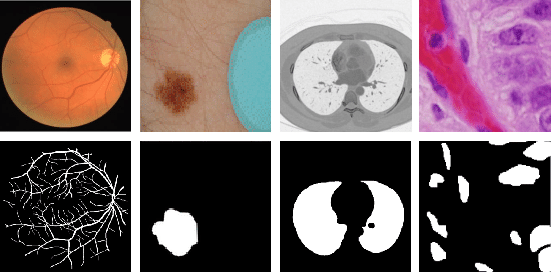
\includegraphics[width=1\linewidth]{recursos/imagens/introduction/medical-image-segmentation.png}
    \label{intro:fig:1}

    Fonte: \cite{Asadi-Aghbolaghi2020}.
\end{figure}

A segmentação de imagens e vídeos é igualmente crucial no desenvolvimento e implementação de sistemas autônomos \citep{Kaymak2019, Liu2020, Pan2020, Teichmann2018}. Nestes sistemas, que abrangem diversas áreas - da indústria ao transporte - a segmentação é frequentemente aplicada a uma variedade de tarefas essenciais.

No setor industrial, por exemplo, máquinas autônomas frequentemente dependem da segmentação para realizar tarefas de controle de qualidade. Isso envolve a análise meticulosa de imagens de produtos em linhas de montagem para identificar, por exemplo, possíveis defeitos de fabricação.

De modo similar, em sistemas de transporte autônomo, como carros completamente automatizados, a segmentação de imagens é vital para garantir a segurança e a eficácia operacional. Tais sistemas utilizam a segmentação para distinguir e identificar precisamente vários elementos em um ambiente de condução - como pedestres, placas de trânsito e sinais de trânsito, conforme desenvolvido por \cite{Lee2018} e \cite{Fleyeh2004}. Esta análise permite que o sistema reaja de maneira adequada a uma variedade de situações de condução e potenciais obstáculos \citep{Lee2018, Fleyeh2004, Pan2020}. A Figura \ref{intro:fig:2} apresenta exemplos de tais aplicações, evidenciando o papel crucial que a segmentação de imagens e vídeos desempenha em sistemas autônomos.

\begin{figure}[H]
    \centering
    \caption{Exemplos de segmentação em sistemas autônomos.}
    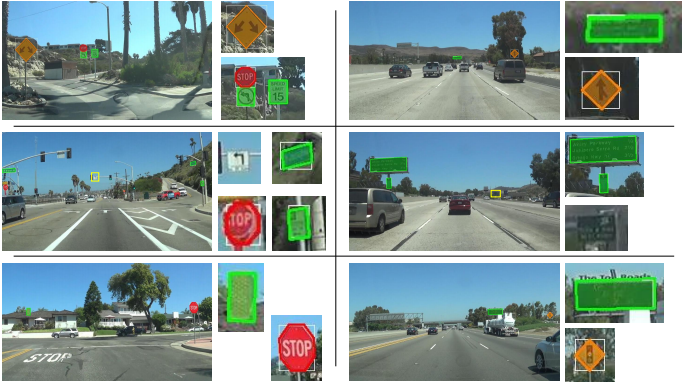
\includegraphics[width=1\linewidth]{recursos/imagens/introduction/placas.png}
    \label{intro:fig:2}

    Fonte: \cite{Lee2018}.
\end{figure}

Embora a segmentação seja um passo essencial no processo de análise de imagens, como mencionado anteriormente, ela não gera diretamente uma ação. Em vez disso, a segmentação muitas vezes faz parte de um protocolo intermediário em fluxos de trabalho que envolvem reconhecimento de imagens ou detecção de objetos.

Um exemplo distinto do papel primordial da segmentação pode ser observado no estudo conduzido por \cite{Carneiro2021}, onde é implementado o método \textit{GrabCut} \citep{rother2004grabcut} para a segmentação de imagens. \textit{GrabCut} é um método de segmentação baseado em grafos, uma abordagem bastante frequente no domínio da segmentação, como explorado por \cite{Yi2012}.

No caso do estudo de \cite{Carneiro2021}, o processo de segmentação é uma etapa prévia à crucial fase de detecção de doenças e pragas em folhas de café. Inicialmente, a segmentação por meio do \textit{GrabCut} é empregada para isolar as folhas de café na imagem. Seguidamente, os resultados desta segmentação servem como base para a detecção mais precisa de possíveis enfermidades ou infestações nessas folhas. A Figura \ref{intro:fig:3} ilustra essa aplicação.

\begin{figure}[H]
    \centering
    \caption{Segmentação feita com \textit{GrabCut}.}
    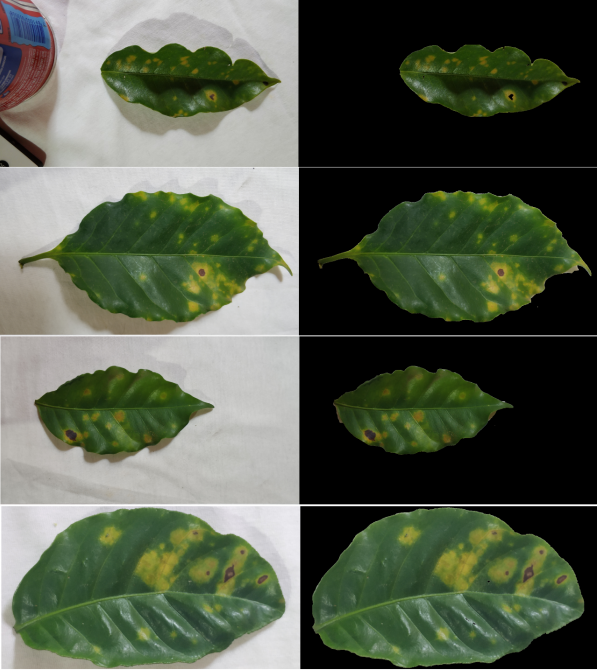
\includegraphics[height=3in]{recursos/imagens/introduction/grabcut.png}

    \label{intro:fig:3}

    Fonte: \cite{Carneiro2021}.
\end{figure}

Este modelo é emblemático de como a segmentação de imagens auxilia em cadeias complexas de processamento em sistemas de visão computacional. Ao facilitar o isolamento preciso de áreas de interesse, a segmentação permite extrair informações mais detalhadas e significativas de imagens, gerando impactos expressivos nos resultados finais. Dessa forma, continua sendo uma ferramenta indispensável em uma grande variedade de aplicações práticas e pesquisas acadêmicas.

Também entre os domínios de aplicação da segmentação de imagens revela-se a área odontológica, com diversas oportunidades e desafios \citep{Ghazvinian2021,Minyoung2020}. Neste ramo, há um contínuo empenho na identificação precisa de todos os componentes presentes na cavidade bucal dos pacientes, variando desde o diagnóstico de condições patológicas, como as cáries, até a avaliação do estado de saúde dos dentes.

Para muitas destas atividades, o diagnóstico é acentuadamente baseado na análise de imagens clínicas, cuja interpretação precisa é fundamental para determinar os próximos passos do tratamento, inclusive a necessidade de dispositivos ortodônticos \citep{Schwendicke2020}. Nessa direção, conforme destacado por \cite{Bansal2021, Nguyen2021} e \cite{Schwendicke2020}, as abordagens baseadas em inteligência artificial têm emergido como soluções promissoras. Ao melhorar a precisão e a velocidade do diagnóstico, elas potencializam o desempenho humano e melhoram os resultados do tratamento.

Um exemplo explícito disso é a aplicação da segmentação de imagens para o reconhecimento de dentes e cáries. Através do uso de métodos de segmentação avançados, é possível isolar e identificar precisamente estas estruturas dentárias e patologias na imagem, facilitando a análise e o diagnóstico subsequente. A Figura \ref{intro:fig:4} apresenta algumas aplicações exemplares da segmentação de imagens em odontologia, demonstrando o potencial deste método para aprimorar a prática clínica.

\begin{figure}[H]
    \centering
    \caption{Exemplo de segmentação na área odontológica.}
    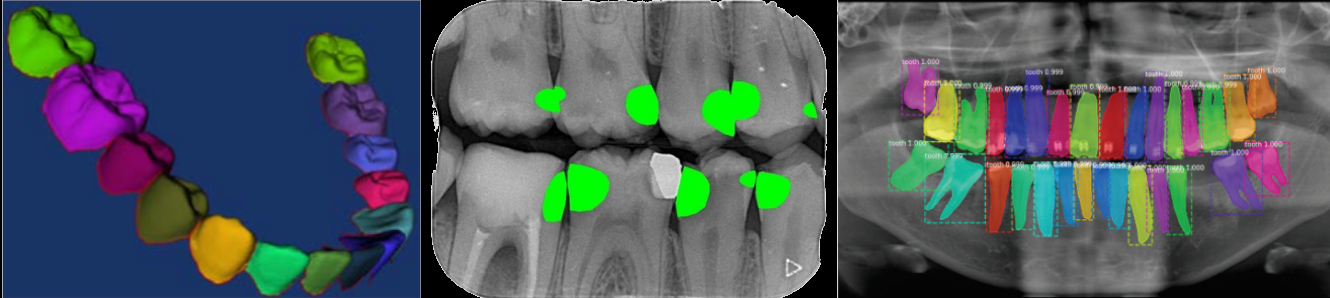
\includegraphics[width=1\linewidth]{recursos/imagens/introduction/odonto_segmentation.png}
    \label{intro:fig:4}

    Fonte: retirado e adaptado de \cite{Shuai2016,Bayrakdar2021,Gil2019}, respectivamente.
\end{figure}

Dentre as abordagens de segmentação, vale dizer que muitos algoritmos foram desenvolvidos para suprir a necessidade de segmentação, dos quais se destacam métodos artesanais (que serão trabalhados no Capitulo \ref{segment}), como os baseados em região ou limiar (Seção \ref{segment:region}), em bordas (Seção \ref{segment:limit}), grafos (Seção \ref{segment:graph}), algorítimos como \textit{Watershed} (Seção \ref{segment:watershed}), \textit{Livewire} (Seção \ref{segment:livewire}) e Superpixel (Seção \ref{segment:superpixel}), além dos agrupamentos (Seção \ref{segment:group}) ou até em métodos mais complexos, devido ao progresso proporcionado pelos avanços de redes neurais, como os algoritmos baseados nessa hipótese (Seção \ref{segment:neural}).

Na medida em que algumas propostas utilizadas em inteligência artificial vêm avançando, observa-se diversos avanços nas áreas de aprendizado profundo, tendo grande destaque e evolução quanto ao âmbito de segmentação de imagens. Esses avanços ocorrem não só devido a um \textit{hardware} com mais capacidade de processamento ou uma maior quantidade de dados disponíveis, mas também por causa da criação de novos algoritmos e abordagens para resolver esses problemas \citep{Szegedy2015} de modo mais adequado.

A partir desses modelos mais modernos que utilizam como recurso o aprendizado profundo, cita-se que estes possuem a capacidade de realizar combinações matriciais com o destaque de características específicas ou até mesmo capacidade de segmentar e propor classes para todos os pixels de uma imagem \citep{Minaee2021}, como é o caso das redes neurais convolucionais (Capitulo \ref{cnn}) e das segmentações semânticas (Capitulo \ref{semantic}).

Com o avanço das técnicas de segmentação mais modernas, tornou-se possível trabalhar com um maior volume de dados presentes nas imagens, abrindo oportunidades para a realização de experimentos relacionados à escala dos objetos presentes na cena e à dimensionalidade preservada pelos modelos. No entanto, mesmo com as abordagens de segmentação mais avançadas, a segmentação de objetos pequenos na imagem ainda representa um grande desafio \citep{Sang2023Small-ObjectAttention, Su2021Small-scaleFusion}.

Outro ponto que pode ser explorados desde os modelos mais profundos que utilizam técnicas para reduzir a dimensionalidade das imagens, até os modelos mais novos com a tarefa de segmentar cada detalhe da imagem, é se os métodos comumente utilizados são os melhores para quesitos de preservação espacial.

Sendo assim, no presente projeto serão listados alguns modelos de algoritmos e \textit{frameworks} conhecidos, dos quais alguns são definidos como estado-da-arte (U-Net, por exemplo), de modo que estes estejam relacionados a segmentações e que seja possível encontrar vantagens, desvantagens e possibilidades de exploração em relação aos mesmos para basear novos experimentos, assim, contribuindo para a evolução científica na esfera de segmentações, principalmente das que fazem uso de aprendizado profundo.

\subsection{Objetivos}
\label{intro:objectives}
O objetivo geral deste trabalho consiste em propor um novo método de \textit{pooling} que, além de reduzir a dimensionalidade, preserva as informações espaciais, visando aprimorar o detalhamento das segmentações. Tal proposta se diferencia dos métodos convencionais de \textit{pooling}, os quais não atendem a esse requisito \citep{Liu2019Multi-LevelNetworks}. Para validar essa abordagem, foram conduzidos experimentos considerando diferentes arquiteturas, desde redes convolucionais convencionais até modelos mais avançados para a segmentação semântica, buscando observar o impacto em diferentes contextos. As principais questões de pesquisa deste trabalho são:

\begin{enumerate}
    \item É possível conceber um método de \textit{pooling} que reduza a dimensionalidade e preserve a espacialidade?
    \item O método de \textit{pooling} proposto é capaz de substituir os métodos convencionais?
    \item Existem diferenças significativas na aplicação do método proposto entre redes convolucionais convencionais e modelos de segmentação semântica?
\end{enumerate}

A primeira questão foi explorada por meio do desenvolvimento de uma proposta de \textit{pooling} denominada \textit{Block-based Principal Component Analysis} (BPCAPooling), a qual será detalhada na Seção \ref{project:bpca}, visando abordar os desafios mencionados nessa questão específica.

O segundo item de pesquisa busca testar o método proposto em comparação com os métodos convencionalmente utilizados para a tarefa de \textit{pooling}. Esta etapa está diretamente relacionada ao terceiro ponto mencionado, o qual visa realizar esses testes em diferentes arquiteturas, desde aquelas mais antigas que introduzem conceitos de \textit{pooling} até arquiteturas mais modernas dedicadas à segmentação detalhada de imagens. Dessa forma, as contribuições pretendidas por esta pesquisa são:

\begin{enumerate}
    \item Desenvolver um novo método de \textit{pooling}.
    \item Avaliar a aplicabilidade do novo método de \textit{pooling} substituindo os métodos convencionais em redes convolucionais tradicionais.
    \item Analisar a eficácia do novo método de \textit{pooling} em substituir os métodos convencionais em modelos de segmentação semântica.
\end{enumerate}


\subsection{Considerações Finais do Capítulo}
\label{intro:end}
Por fim, nos capítulos seguintes, assuntos relacionados à apresentação de conceitos de redes neurais profundas e redes neurais convolucionais serão tratadas no Capítulo \ref{deep}. Após, será discorrido sobre as técnicas que tradicionalmente são utilizadas para atividades de segmentação no Capítulo \ref{segment}, acompanhada de segmentações que são fruto do advento das redes convolucionais e aprendizado profundo, tratando da segmentação semântica (Capítulo \ref{semantic}), para quê, finalmente sejam apresentados os detalhes da metodologia proposta nesse trabalho de forma clara no Capítulo \ref{project}.  Finalmente, o Capítulo \ref{results} apresentará os resultados e discussões e o Capitulo \ref{conclusion} apresenta algumas considerações finais do trabalho.